\section{Tensor Trifocal: detalhamento da abordagem de Nistér e Schaffalitzky.}

Para abordar um problema trifocal, primeiro \cite{2503343} desenvolvem uma abordagem num sistema bifocal para determinação da rotação e da translação (supondo qua a calibração já seja conhecida) da segunda câmera em relação à primeira, considerando duas imagens de quatro pontos em 3D. Eles demonstram que os epipolos de cada imagem estão restritos a se alojarem numa curva de grau 10, a chamada curva décica, bem como desenvolvem um método para a obtenção dessa curva. De posse dos epipolos, definem a geometria epipolar, resgatam a segunda câmera em relação à primeira e fazem a reconstrução 3D. Com os pontos em 3D e a terceira imagem, resgatam a terceira câmera em relação à primeira. Utilizam essa teoria para desenvolver o que chamaram de solução mais eficiente para época (2006), o notório desafio de estabelecer as poses das câmeras num sistema com três imagens. Vamos incluir os detalhes mais importantes na reprodução desse artigo. 

\begin{figure}[!htb]
\centering
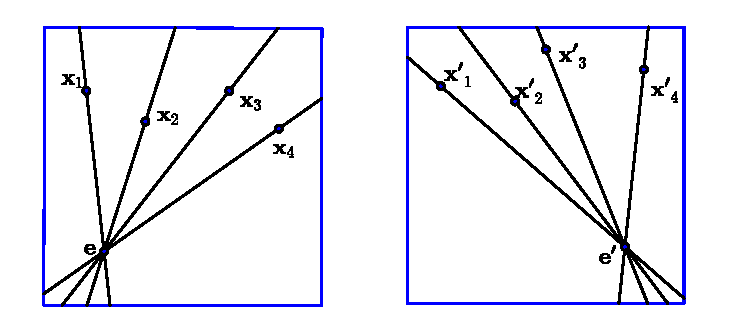
\includegraphics[scale=.85]{retas-epipolares}
\caption{\textit{Feixe de retas passando pelo epipolo em cada imagem, relacionadas duas a duas por uma homografia.}}
\label{retas-epipolares}
\end{figure}

\subsection{O teorema 1.} 

Uma das primeiras afirmações importantes do artigo é de as retas epipolares numa imagem estão homograficamente relacionadas com as retas epipolares na segunda imagem. Dados $n$ correspondências de pontos em duas imagens, a \textit{restrição epipolar} \citep{faugeras93three} pode ser expressa como: os parâmetros projetivos das $n$ retas ligando o epipolo ${\bf e}$ aos pontos ${\bf x}_i$ na primeira imagem, estão homograficamente relacionados com os parâmetros projetivos das $n$ retas ligando o epipolo ${\bf e'}$ aos pontos ${\bf x'}_i$ na segunda imagem. Ou seja, temos uma homografia 1D que relaciona o feixe de retas através ${\bf e}$ com o feixe de retas através ${\bf e'}$ chamada \textit{homografia da reta epipolar}. Podemos visualizar essa situação na figura \ref{retas-epipolares}.


\subsubsection{Detalhamento: a homografia da reta epipolar.} 


Supondo os epipolos na origem do plano de cada imagem, com as retas epipolares passando pelo epipolo, cada reta pode ser parametrizada através do ângulo que ela forma com o eixo das abscissas, denominados $\alpha_1$ e $\alpha_2$ na primeira e segunda imagens respectivamente.
A homografia da reta epipolar pode ser representada pela equação de uma hipérbole alinhada aos eixos perpendiculares, conforme descrito em \cite{Fabbri:Kimia:IJCV2015}.

\begin{equation}\label{eq.hiperbole}
a\,x\,y+b\,x+c\,y+d=0 \qquad \text{ou} \qquad y=\frac{-b\,x-d}{a\,x+c},
\end{equation} 
onde $x=tan\,\alpha_1$ e $y=tan\,\alpha_2$. 

Vemos na figura \ref{fig.reta-epipolar} que cada reta epipolar fica definida por um ponto no eixo da tangente, $(1,tan\,\alpha_1)$ na primeira imagem e $(1,tan\,\alpha_2)$ na segunda, onde consideramos o círculo trigonométrico de raio $1$. Usando esses pontos, a equação da hipérbole pode ser escrita na forma

\begin{equation}\label{eq.homo-reta-epi}
(1\,,\,tan\,\alpha_1)
\overbrace{
\begin{bmatrix}
d&c\\
b&a
\end{bmatrix}
}^{H}
\begin{pmatrix}
1\\
tan\,\alpha_2
\end{pmatrix}
=0,
\end{equation}
sendo 
$\begin{bmatrix}d&c\\b&a\end{bmatrix}$ a homografia procurada.

O problema é que a equação \ref{eq.homo-reta-epi} não está definida para retas epipolares verticais, pois utilizamos a tangente, e uma saída é parametrizar cada reta através da própria definição de tangente, pois assim temos uma representação isotrópica \footnote{É o que se diz de um corpo que, em todas as direções, apresenta as mesmas propriedades ópticas.} para as retas:

\begin{equation}\label{eq.tan.alpha1-2}
x=tan\,\alpha_1=\frac{sen\,\alpha_1 }{cos\,\alpha_1} \qquad \text{e} \qquad y=tan\,\alpha_2=\frac{sen\,\alpha_2}{cos\,\alpha_2}.
\end{equation} 

Desta forma, substituindo \ref{eq.tan.alpha1-2} em \ref{eq.hiperbole} e multiplicando por $cos\,\alpha_1\,cos\,\alpha_2$ temos

\begin{equation*}
a\,sen\,\alpha_1\,sen\,\alpha_2+b\,sen\,\alpha_1\,cos\,\alpha_2+c\,cos\,\alpha_1\,sen\,\alpha_2+d\,cos\,\alpha_1\,cos\,\alpha_2=0.
\end{equation*}

\begin{figure}[!htb]
\centering
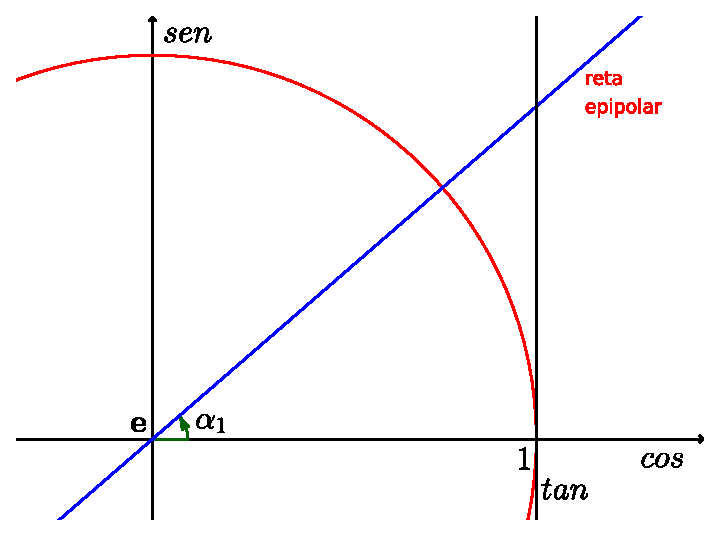
\includegraphics[scale=1]{reta-epipolar-alpha1}
\caption{\textit{Plano da imagem centrado em ${\bf e}$ com a reta epipolar parametrizada por $\alpha_1$.}}
\label{fig.reta-epipolar}
\end{figure}

Com essa conversão, deixamos de parametrizar as retas epipolares pelo eixo da tangente e passamos a parametrizar pelo círculo trigonométrico. Aqui temos um argumento para contagem dos graus de liberdade para fixarmos a relação entre retas epipolares, pois devemos determinar os dois epipolos (duas variáveis cada totalizando quatro graus de liberdade), e mais a matriz que representa a homografia (quatro variáveis mas apenas três graus de liberdade utilizando uma variável para fixar a escala). Portanto, precisamos de no mínimo sete restrições para determinarmos a relação entre duas imagens na geometria epipolar. 

Na nossa abordagem, consideramos o círculo trigonométrico com raio $1$ mas podemos estipular raios arbitrários $r_1$ e $r_2$ em cada uma das imagens que ajuda a garantir estabilidade numérica para a determinação dos coeficientes. Assim, obtemos a equação:

\begin{equation*}
a\,r_1\,sen\,\alpha_1\,r_2\,sen\,\alpha_2+b\,r_1\,sen\,\alpha_1\,r_2\,cos\,\alpha_2+c\,r_1\,cos\,\alpha_1\,r_2\,sen\,\alpha_2+d\,r_1\,cos\,\alpha_1\,r_2\,cos\,\alpha_2=0.
\end{equation*}

Em resumo, as vantagens dessa última representação é ser isotrópica e ter boa estabilidade numérica para escolhas convenientes de $r_1$ e $r_2$, e novamente  na representação matricial:

\begin{equation*}
(r_1\,cos\,\alpha_1\,,\,r_1\,sen\,\alpha_1)
\begin{bmatrix}
d&c\\
b&a
\end{bmatrix}
\begin{pmatrix}
r_2\,cos\,\alpha_2\\
r_2\,sen\,\alpha_2
\end{pmatrix}
=0
\end{equation*}

\subsubsection{Detalhamento: segunda abordagem para mapeamento entre retas epipolares.}\label{sec.homografia-reta-epipolar}


Uma outra forma de pensar sobre essa homografia, encontrada em \cite{Hartley2004}, é considerando que as retas epipolares estão perspectivamente relacionadas com centro em um ponto $Q$ na reta base, conforme a figura \ref{fig.retas-epi-hartley}.

\begin{figure}[!htb]
\centering
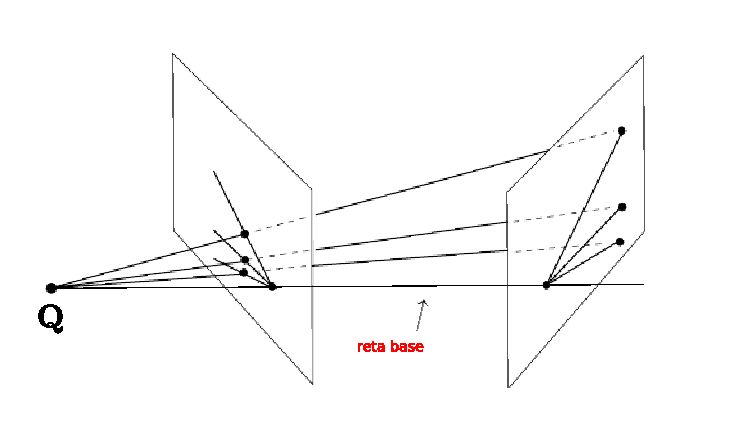
\includegraphics[scale=1]{retas-epipolares-hartley}
\caption{\textit{Retas epipolares com perspectiva centrada em $Q$ na reta base.}}
\label{fig.retas-epi-hartley}
\end{figure}


Suponha que $\lightrgb$ e $\lightrgb'$ sejam duas retas epipolares correspondentes, e ${\bf m}$ é uma reta qualquer que não passa pelo epipolo $\e$. O produto vetorial 

\begin{equation}
{\bf m}\times\lightrgb=\x\qquad\text{ou}\qquad\,[{\bf m}]_\times\,\lightrgb=\x,
\end{equation}
nos fornece o ponto $\x$ de interseção entre essas retas. Pela subseção \ref{sec.matriz-F} temos que

\begin{equation*}
\lightrgb'=F\,\x,
\end{equation*} 
assim, $\lightrgb$ é mapeada a $\lightrgb'$ através da relação 

\begin{equation*}
\lightrgb'=F\,[{\bf m}]_\times\,\lightrgb
\end{equation*}


Uma boa escolha para ${\bf m}$ é a reta $\e$, já que

\begin{equation*}
{\bf m}^\top\e=\e^\top\e\neq0,
\end{equation*}
então $\e$ é uma reta que não passa pelo epipolo $\e$ como desejado. Assim, a homografia da reta epipolar pode ser escrita como 

\begin{equation*}
\lightrgb'=F\,[\e]_\times\,\lightrgb.
\end{equation*}
O argumento é análogo para o mapeamento da segunda imagem para a primeira,

\begin{equation*}
\lightrgb=F^\top [\e']_\times\,\lightrgb'.
\end{equation*}\\

\subsection{Dedução da IAC.}

Uma ferramenta algébrica bastante utilizada nessa abordagem de \citep{2503343} é a imagem da cônica absoluta (IAC em inglês) denotada por ${\bf \omega}$. Como a abordagem assume que as câmeras são calibradas, vamos mostrar que é possível obter a IAC em função da matriz de calibração da câmera $K$.

\subsubsection{Detalhamento: a matriz de calibração, a imagem da cônica absoluta e a imagem da cônica dual absoluta.}

 Inicialmente, vamos determinar a homografia que faz o mapeamento do plano no infinito $\bpi_\infty$ para o plano da imagem na câmera. Se $\X_\infty\in\bpi_\infty$ então pode ser escrito na forma

\begin{equation*}
\X_\infty=({\bf d}^\top,0)^\top
\end{equation*} 
e é projetado por uma câmera geral $P=K\,[R|{\bf t}]$ como

\begin{equation*}
\begin{array}{rcl}
\x&=&P\,\X_\infty\\
&=&K\,[R|{\bf t}]\,({\bf d}^\top,0)^\top\\
&=&K\,R\,{\bf d}.
\end{array}
\end{equation*}
Portanto temos a relação

\begin{equation*}
\x=H\,{\bf d}
\end{equation*}
onde $H=K\,R$. Como a cônica absoluta $\Omega_\infty$ está contida no plano no infinito (contém pontos no infinito), ela pode ser projetada sob a homografia $H$ para computarmos sua imagem.
Sob uma homografia de ponto $\x\rightarrow H\,\x$, uma cônica se transforama de acordo com $C\rightarrow H^{-\top} C\,H^{-1}$, conforme a subseção \ref{sec.trans-proj-H}. De acordo com a subseção \ref{sec.con-absoluta} $C=\Omega_\infty =I$, daí temos

\begin{equation*}
\begin{array}{rcl}
{\bf \omega}&=&H^{-\top}\Omega_\infty\,H^{-1}\\
&=&(K\,R)^{-\top}\,I\,(K\,R)^{-1}\\
&=&K^{-\top}R^{-\top}R^{-1}K^{-1}\\
&=&K^{-\top}K^{-1}
\end{array}
\end{equation*}
pois $R$ é uma matriz de rotação e portanto satisfaz $R^{-\top}R^{-1}=I$. Assim, de posse de uma câmera calibrada é simples obter a IAC.

Analogamente ao que é feito na subseção \ref{sec.conica-dual}, podemos definir a imagem dual da cônica absoluta (sigla DIAC em inglês), denotada por $\omega^*$, a partir de $\omega$ como

\begin{equation*}
\omega^*=\omega^{-1}=K\,K^\top.
\end{equation*}
Esta é uma cônica definida por retas e é a imagem da quádrica dual absoluta ${\tt Q^*_\infty}$, definida na subseção \ref{sec.quadrica-dual-abs}. A imagem é dada por

\begin{equation*}
\omega^*=P\,{\tt Q^*_\infty}P^\top,
\end{equation*}
conforme a subseção \ref{sec.proj-quadricas}.\\

\subsection{O teorema 2.}\label{sec.teorema-2}


Para a correspondência entre retas tangentes às duas cônicas ${\bf \omega}$ e ${\bf \omega'}$ podemos utilizar a restrição \textit{Kruppa}: as duas retas tangentes à ${\bf \omega}$ e passando por $\e$, estão relacionadas por uma homografia de reta epipolar às duas tangentes à ${\bf \omega'}$ passando por $\e'$. Na figura \ref{epipolar-kruppa} podemos observar as restrições epipolar e Kruppa simultaneamente.

\begin{figure}[!htb]
\centering
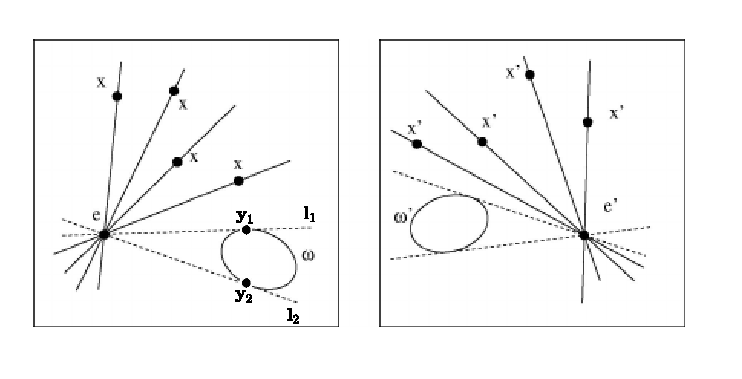
\includegraphics[scale=1.2]{restricao-epipolar-kruppa}
\caption{\textit{Retas epipolares tangentes às cônicas ${\bf \omega}$ e ${\bf \omega'}$.}}
\label{epipolar-kruppa}
\end{figure}

A restrição Kruppa foi originalmente introduzida por \cite{faugeras92} e está relacionada com uma cônica contida num plano no espaco 3D e suas imagens nas câmeras $1$ e $2$, e é válida para cônicas gerais, mas aqui no nosso caso vamos tratar especificamente da cônica absoluta $\Omega_\infty$ contida no plano infinito $\bpi_\infty$ no espaco, e as imagens da cônica absoluta (IAC) ${\bf \omega}$ e ${\bf \omega'}$.


\subsubsection{Detalhamento: as restrições Kruppa.}


 Sendo ${\bf \omega}^*$ e ${{\bf \omega}^*}'$ as respectivas cônicas duais (DIAC), considere um plano passando pelo centro das duas câmeras e tangenciando essa cônica $\Omega_\infty$ no espaco. Por construção, esse plano vai projetar uma reta epipolar em cada imagem onde cada reta será tangente às imagens ${\bf \omega}$ e ${\bf \omega'}$ da cônica $\Omega_\infty$, observado na figura \ref{geometria-kruppa}. E suponha ainda que $\lightrgb_1$ e $\lightrgb_2$ sejam as retas tangentes à cônica ${\bf \omega}$ na primeira imagem conforme a figura \ref{epipolar-kruppa}. Com essas duas retas tangentes podemos construir uma cônica degenerada $D$ (posto $1$ ou $2$) da seguinte maneira:  

\begin{equation}\label{eq.def.con.deg}
D=[\e]_\times\,{\bf \omega}^*\,[\e]_\times \qquad \text{ou, como outra construção} \qquad D=\lightrgb_1\,\lightrgb_2^\top + \lightrgb_2\,\lightrgb_1^\top
\end{equation}

Para mostrar que $D$ é uma cônica (ponto) temos que verificar que é válida a relação $\y_1^\top D\,\y_1=0$, onde $\y_1\in\lightrgb_1$.

\begin{equation*}
\begin{array}{rcll}
\y_1^\top\,D\,\y_1&=&\y_1^\top [\e]_\times\,{\bf \omega}^*\,[\e]_\times\,\y_1&\\
&=&([\e]^\top_\times\,\y_1)^\top {\bf \omega}^*\,[\e]_\times\,\y_1&\\
&=&\lightrgb_1^\top {\bf \omega}^*\,\lightrgb_1& \qquad\text{pois}\qquad\lightrgb_1=\e\times\y_1\\
&=&0&
\end{array}
\end{equation*}
onde a última passagem segue do fato de ${\bf \omega}^*$ ser dual. Observe que usamos $[\e]^\top_\times\,\y_1=[\e]_\times\,\y_1$ quando na verdade $[\e]^\top_\times=-[\e]_\times$, mas aqui a diferença de escala é irrelevante. Analogamente, para a segunda definição de $D$:

\begin{figure}[!htb]
\centering
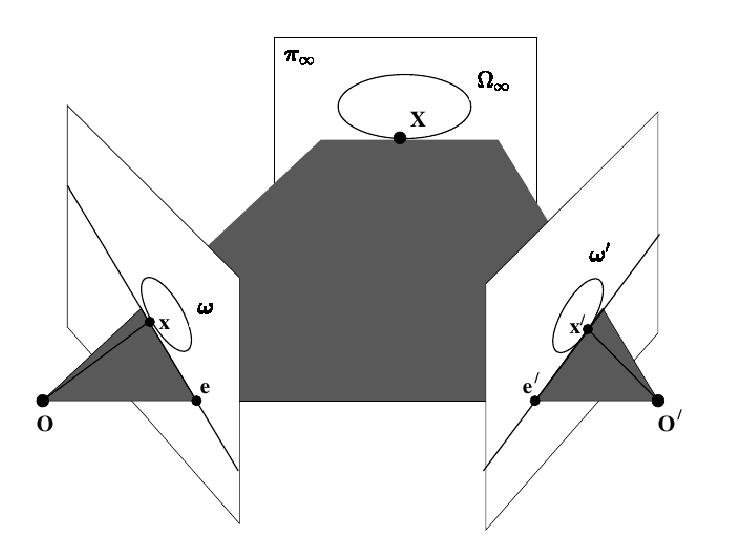
\includegraphics[scale=1.1]{geometria-kruppa}
\caption{\textit{Um plano epipolar tangenciando uma cônica no espaco 3D projeta retas epipolares que tangenciam as cônicas nos planos das imagens}.}
\label{geometria-kruppa}
\end{figure}

\begin{equation*}
\y_1^\top\,D\,\y_1=\y_1^\top \lightrgb_1\,\lightrgb_2^\top + \lightrgb_2\,\lightrgb_1^\top\y_1=0
\end{equation*}
pois como $\y_1\in\lightrgb_1$ então $\y_1^\top \lightrgb_1=\lightrgb_1^\top\y_1=0$. Observamos que o desenvolvimento anterior é análogo para $\lightrgb_2$.

Na segunda imagem, analogamente à primeira, $D'=[\e']_\times\,{{\bf \omega}^*}'\,[\e']_\times$ e se transforma de acordo com a regra $D'=H_\infty^{-\top}D\,H_\infty^{-1}$ na subseção \ref{sec.trans-proj-H}. O símbolo $\infty$ se deve ao fato de que a homografia foi deduzida de maneria similar àquela da subseção  \ref{sec.homografia}, apenas com a diferença de ter sido com base no plano no infinito. Assim:

\begin{equation}\label{eq.kruppa}
\begin{array}{rcll}
[\e']_\times\,{{\bf \omega}^*}'\,[\e']_\times&=&D'&\\
&=&H_\infty^{-\top}D\,H_\infty^{-1}&\\
&=&H_\infty^{-\top}[\e]_\times\,{\bf \omega}^*\,[\e]_\times\,H_\infty^{-1}&\qquad\text{pois}\qquad D=[\e]_\times\,{\bf \omega}^*\,[\e]_\times\\
&=&F\,\omega^* F^\top,&
\end{array}
\end{equation}
onde $F=H_\infty^{-\top}\,[\e]_\times$ conforme a subseção \ref{sec.matriz-F}. 


Da relação \ref{eq.kruppa} são extraídas as duas equações quadráticas independentes eliminando-se o fator de escala, onde tais equações são conhecidas como as restrições de Kruppa. 


\subsection{Mudança de coordenadas projetivas.}

De acordo com \cite{kneebone}, podemos escolher as coordenadas projetivas de forma que os quatro pontos também tenham as mesmas coordenadas em cada imagem. Ou seja, podemos assumir que ${\bf x}_i = {\bf x'}_i$ pensando nos dois planos de imagem como registrados no mesmo sistema de coordenadas. Vejamos como isso pode ser feito.

\subsubsection{Detalhamento: corregistro de pontos pertencentes a diferentes planos de imagem.}\label{sec.corregistro-pontos}
Suponha a existência de pontos em correspondêcia em dois planos de imagem relacionados por uma transformação projetiva $\x'=H\,\x$, onde $\x\in {\mathbb{P}^2}$ e $\x'\in {\mathbb{P'}^2}$. Fazendo as seguintes mudanças de coordenadas projetivas

\begin{equation}\label{eq.igualando-coordenadas}
\begin{array}{rcl}
\overline{\x}\,&=&I\,\x\\
\overline{\x}'&=&H^{-1}\x',
\end{array}
\end{equation}
temos que $\x=\overline{\x}$ e $\x'=H\,\overline{\x}'$. Substituindo essas duas últimas igualdades em $\x'=H\,\x$ temos

\begin{equation*}
\begin{array}{rcll}
\x'&=&H\,\x&\Rightarrow\\
H\,\overline{\x}'&=&H\,\overline{\x}&\Rightarrow\\
\overline{\x}'&=&H^{-1}H\,\overline{\x}&\Rightarrow\\
\overline{\x}'&=&\overline{\x}.&
\end{array}
\end{equation*}
Cabe ressaltar que as mudanças de coordenadas em \ref{eq.igualando-coordenadas} não altera nosso desenvolvimento, já que aqui nos interessa propriedades que são invariantes sob transformações projetivas, como tangências, interseções e raz\~ao cruzada.

\subsection{O teorema 3.}\label{sec.teorema-3}

Aplicando as mudanças de coordenadas descritas na subsec\~ao \ref{sec.corregistro-pontos} nos quatro pontos e nos epipolos, a restrição epipolar pode ser convertida em: os epipolos ${\bf e}$ e ${\bf e'}$ juntamente com os quatros pontos, que obedecem a restrição epipolar, devem estar alojados numa cônica $B$ e, reciprocamente, dois epipolos ${\bf e}$ e ${\bf e'}$ que são concônicos com quatro pontos na imagem satisfazem a restrição epipolar. 

\subsubsection{Detalhamento: argumentação do teorema.}

Pela subseção \ref{sec.definicao-conica}, uma cônica fica determinada por cinco pontos, como temos quatro pontos na imagem vamos deixar a cônica $B$ na dependência de $\e$ (o quinto ponto necessário). Analogamente, o epipolo $\e'$ também define uma cônica com os quatro pontos na imagem, digamos $B'$. Pela subsec\~ao \ref{sec.homografia-reta-epipolar}, existe a homografia da reta epipolar que relaciona essas quatro retas de cada feixe passando por $\e$ e $\e'$. Pelo teorema de Steiner, \citep{kneebone}, se dois feixes de retas passando por $\e$ e $\e'$ estão homograficamente relacionados, o ponto de interseção entre retas correspondentes desses feixes descreve uma cônica que passa por $\e$ e $\e'$. Portanto $B=B'$ e todos os seis pontos em questão são concônicos.


Reciprocamente, pelo teorema de Chasles em \citep{kneebone}, se quatro pontos $\x_i$ numa cônica formam um feixe de retas concorrentes em um quinto ponto $\e\in B$, a razão cruzada entre as quatro retas não depende da posição de $\e$. Assim, a razão cruzada  do feixe concorrente em $\e$ é igual a do feixe concorrente em $\e'$. Pela subseção \ref{sec.geometria-1D}, a razão cruzada num feixe de retas é igual à razão cruzada entre os quatro pontos de interseção de uma reta qualquer com o feixe. Pelo corolário ainda na subseção \ref{sec.geometria-1D}, dois conjuntos de quatro pontos colineares têm a mesma razão cruzada se, e somente se, correspondem sob uma homografia.  


Esta cônica $B=B(\e)$ será bastante importante durante a abordagem pois, se os dois epipolos são concônicos com os quatro pontos na imagem, figura \ref{pontos-conconicos}, existe uma \textit{única} homografia de reta epipolar que faz a relação das quatro retas através ${\bf e}$ com as quatro retas através ${\bf e'}$. 

\begin{figure}[!htb]
\centering
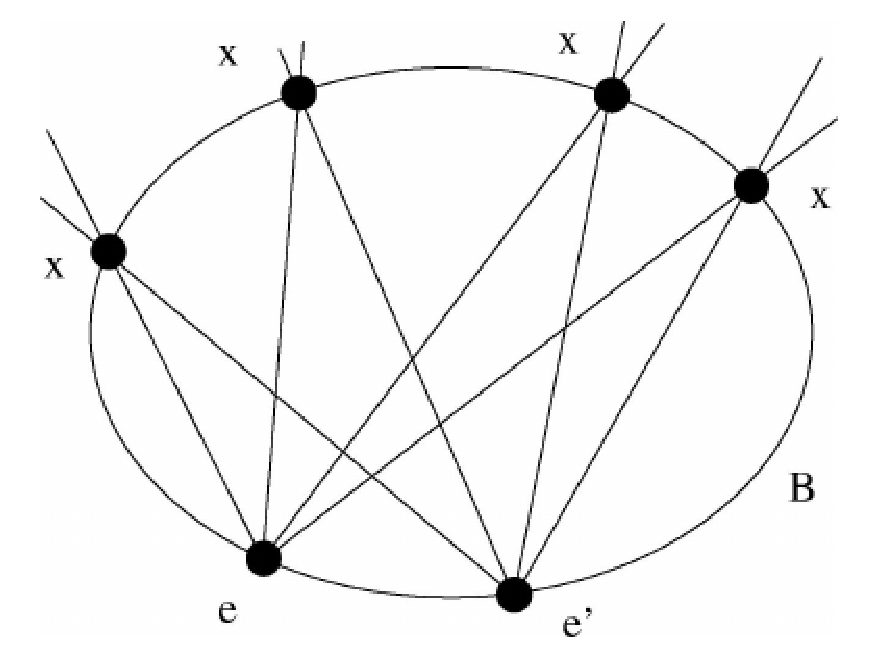
\includegraphics[scale=.85]{pontos-conconicos}
\caption{\textit{Epipolos concônicos com os quatro pontos na imagem produzem homografia única.}}
\label{pontos-conconicos}
\end{figure}

\subsection{O teorema 4.}

Note que podemos parametrizar o feixe de retas passando por ${\bf e'}$ (ou ${\bf e}$) por pontos pertencentes à cônica $B$, pois retas correspondentes nos dois feixes intersectam $B$ no mesmo ponto. Desta forma, o teorema 4 é anunciado como: as restrições de calibração são equivalentes à condição de que as duas retas tangentes à cônica ${\bf \omega}$ e passando por ${\bf e}$, intersectam a cônica $B$ nos mesmos dois pontos adicionais que as retas tangentes à ${\bf \omega'}$ e passando por ${\bf e'}$. 

\subsubsection{Detalhamento: argumentação do teorema.}
Na subseção \ref{sec.teorema-2}, vimos que as duas retas tangentes à conica $\omega$ estão projetivamente relacionadas com as duas tangentes à cônica $\omega'$. Pelo teorema de Steiner, na subseção \ref{sec.teorema-3}, o ponto de interseção entre duas retas correspondentes, em dois feixes homograficamente relacionados, descrevem uma cônica. Assim, as retas tangentes à cônica $\omega$ se intersectam às retas tangentes à cônica $\omega'$ em dois pontos adicionais sobre a cônica $B$. 

Isto é, as projeções de ${\bf \omega}$ e ${\bf \omega'}$ em $B$, através dos respectivos epipolos, devem coincidir. Essa construção geométrica pode ser visualizada na figura \ref{omega-B} e será a fundação para o resto da abordagem. 

\begin{figure}[!htb]
\centering
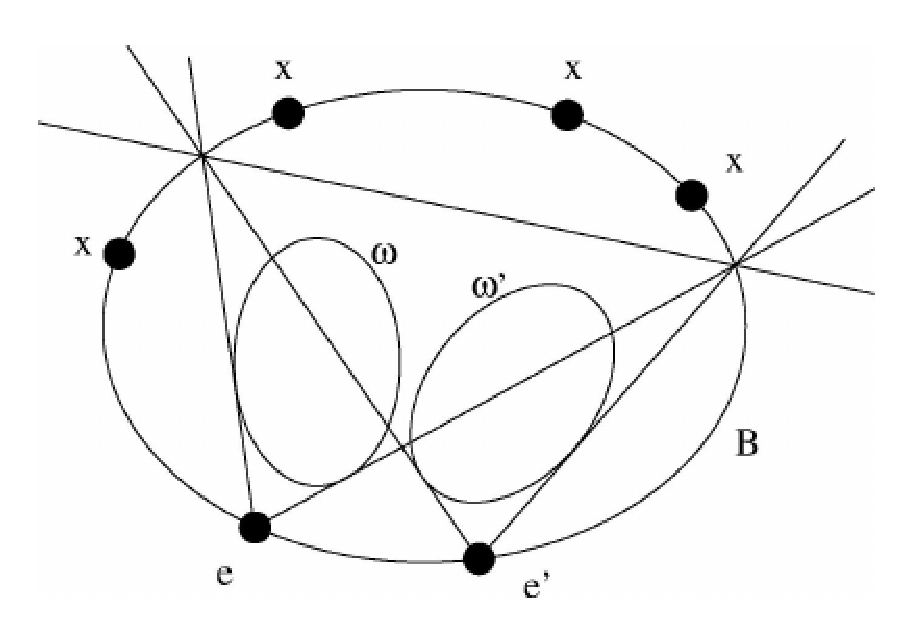
\includegraphics[scale=.85]{projecao-omega-B}
\caption{\textit{Os pontos de interseção das tangentes com a cônica $B$ coincidem, ocasionando a coincidência das projeções das cônicas ${\bf \omega}$ e ${\bf \omega'}$ na cônica $B$.}}
\label{omega-B}
\end{figure}

\subsection{O teorema 5.}

A demonstração desse teorema é dada em \cite{2503343} e vamos incluir alguns detalhes.
Podemos pensar na representação da projeção de  ${\bf \omega}$ e ${\bf \omega'}$ em $B$ como a reta que liga os dois pontos de interseção das tangentes com $B$. Essa reta que liga os dois pontos de interseção, de acordo com a projeção de ${\bf \omega}$ através do epipolo ${\bf e}$ é representada por $({\bf \omega}\diamond B)\,{\bf e}$, e a cônica $({\bf \omega}\diamond B)$ é definida como:

\begin{equation}\label{eq.conica-diamond}
(\omega \diamond B)\equiv 2\,B\,\omega^*B - tr(\omega^*\,B)\,B,
\end{equation}
onde $\omega^*$ é a matriz adjunta de $\omega$.

A equação \ref{eq.conica-diamond} é uma fórmula projetivamente invariante de uma cônica. Para ver isso, basta tomar uma configuração genérica para as cônicas $B$ e $\omega^*$, digamos

\begin{equation*}
B=
\begin{bmatrix}
a&b&c\\
b&d&e\\
c&e&f
\end{bmatrix}
\qquad\text{e}\qquad
\omega^*=
\begin{bmatrix}
g&h&i\\
h&j&l\\
i&l&m
\end{bmatrix},
\end{equation*} 
e efetuar as multiplicações constantes na equação \ref{eq.conica-diamond}. Lembrando que o traço de uma matriz é definido pela soma dos elementos da diagonal principal, o resultado das multiplicações é uma matriz simétrica, que pela subseção \ref{sec.definicao-conica}, representa uma cônica. Pela subseção \ref{sec.trans-proj-H}, uma homografia leva uma cônica em outra cônica, a qual mantém as características invariantes sob transformação projetiva.

\subsubsection{Representação canônica de uma cônica.}

Como vimos na subseção \ref{sec.espaco-P2}, o plano projetivo $\mathbb{P}^2$ tem seus pontos representados por vetores homogêneos com três componentes. Da algebra linear sabemos que o espaço $\mathbb{R}^3$ também tem seus pontos representados por vetores com três componentes. Portanto, existe uma analogia entre as representações mesmo que no plano projetivo a relação entre vetores e pontos não seja biunívoca como em $\mathbb{R}^3$. Da mesma forma que podemos escolher a base canônica para representar vetores em $\mathbb{R}^3$, fazendo a devida transformação projetiva do sistema de coordeandas, podemos escolher uma base para representação do plano projetivo incluindo um \textit{vetor unitário} ${\bf u}=(1,1,1)$. Assim, cada ponto em $\mathbb{P}^2$ pode ser representado em termos da base \{$\x_1=(1,0,0),\x_2=(0,1,0),\x_3=(0,0,1),{\bf u}=(1,1,1)$\} onde os três primeiros vetores são chamados {\it pontos de referência}. Para detalhes ver \citep{kneebone}.

Os pontos de referência, que são linearmente independentes, formam os vértices de um triângulo chamado \textit{triângulo de referência}, com o ponto unitário no interior do triângulo. Esse triângulo vai servir como uma base para a representação do plano projetivo, conforme a figura \ref{fig.triangulo-referencia}. Por exemplo, representando um ponto qualquer por $\x=(x,y,z)^\top$ e uma reta qualquer por $\lightrgb=(a,b,c)^\top$ a reta determinada pelos pontos $\x_1$ e ${\bf u}$ tem equação $z-y=0$.

\begin{figure}[!htb]
\centering
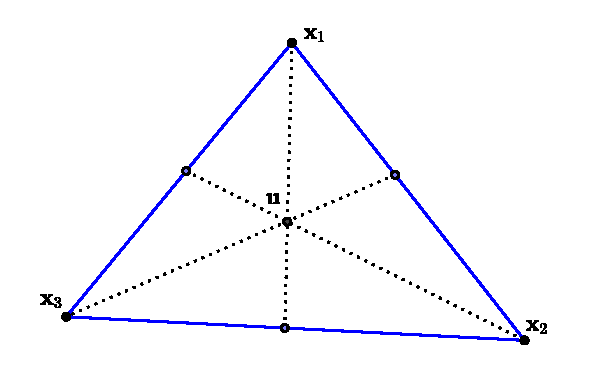
\includegraphics[scale=1]{triangulo-referencia}
\caption{{\it Triângulo de referência com vértices determinados por três vetores que, juntamente com o vetor unitário, servem de base para representação do plano projetivo.}}
\label{fig.triangulo-referencia}
\end{figure}

Pois, se $\x_1\in\lightrgb$ e ${\bf v}\in\lightrgb$ então

\begin{equation}\label{eq.exemplo-tri-referencia}
\lightrgb^\top{\bf u}=0\Rightarrow a+b+c=0\qquad\text{e}\qquad\lightrgb^\top\x_1=0\Rightarrow a=0.\qquad\text{Assim,}\quad c=-b.
\end{equation}

Dado um ponto qualquer $\x\in\lightrgb$ a equação da reta fica

\begin{equation*}
\lightrgb^\top\x=0\Rightarrow a\,x+b\,y+c\,z=0,
\end{equation*}
usando \ref{eq.exemplo-tri-referencia} temos que

\begin{equation*}
-c\,y+c\,z=0\Rightarrow z-y=0,
\end{equation*}
já que $c=0$ pois do contrário $\lightrgb$ representaria um ponto no infinito.

Existem algumas formas padronizadas pelas quais a representação de uma cônica $C$ pode ser simplificada através da escolha conveniente de uma estrutura de referência. Umas dessas escolhas é tomar o triângulo de referência como tendo dois de seus lados tangentes à cônica, e o terceiro lado como reta polar em relação ao vértice oposto, e escolher um ponto  da cônica como ponto unitário. Ver figura \ref{fig.conica-tri-referencia}.

\begin{figure}[!htb]
\centering
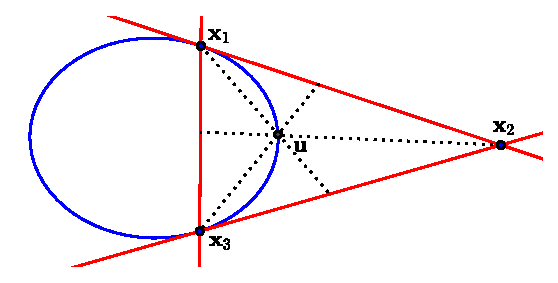
\includegraphics[scale=1]{conica-tri-referencia}
\caption{{\it Uma cônica $C$ numa relação polo-polar com um triângulo de referência que representa o plano projetivo $\mathbb{P}^2$}.}
\label{fig.conica-tri-referencia}
\end{figure}

Como vimos na subseção \ref{sec.definicao-conica}, uma cônica $C$ pode ser representada na forma matricial com coordenadas homogêneas como

\begin{equation*}
\begin{pmatrix}
x&y&z
\end{pmatrix}
\begin{bmatrix}
a&b/2&c/2\\
b/2&d&e/2\\
c/2&e/2&f
\end{bmatrix}
\begin{pmatrix}
x\\
y\\
z
\end{pmatrix}
=0
\end{equation*}
ou através da equação

\begin{equation*}
a\,x^2+b\,x\,y+d\,y^2+c\,x\,z+e\,y\,z+f\,z^2=0.
\end{equation*}

Supondo que a cônica passe pelos pontos $\x_1=(1,0,0)^\top$ e $\x_3=(0,0,1)^\top$ temos que

\begin{equation*}
\x_1\in C\Rightarrow a=0\quad\text{e}\quad\x_3\in C\Rightarrow f=0,
\end{equation*}
daí a equação da cônica será 

\begin{equation}\label{eq.reducao-parcial-conica}
d\,y^2+b\,x\,y+c\,x\,z+e\,y\,z=0.
\end{equation}

Consirede a reta $\lightrgb=(l_1,l_2,l_3)^\top$ que passa pelos pontos $\x_1$ e $\x_3$,

\begin{equation*}
\lightrgb^\top\x_1=
\begin{pmatrix}
l_1&l_2&l_3
\end{pmatrix}
\begin{pmatrix}
1\\
0\\
0
\end{pmatrix}
=0
\Rightarrow l_1=0,
\end{equation*} 

\begin{equation*}
\lightrgb^\top\x_1=
\begin{pmatrix}
l_1&l_2&l_3
\end{pmatrix}
\begin{pmatrix}
0\\
0\\
1
\end{pmatrix}
=0
\Rightarrow l_3=0,
\end{equation*} 
e portanto $\lightrgb=(0,l_2,0)^\top$.

Observando que $\lightrgb$ está numa relação polo-polar com o ponto $\x_2$, pela subseção \ref{sec.polo-polar} temos que $C\,\x_2=\lightrgb$, daí

\begin{equation*}
\begin{bmatrix}
a&b/2&c/2\\
b/2&d&e/2\\
c/2&e/2&f
\end{bmatrix}
\begin{pmatrix}
0\\
1\\
0
\end{pmatrix}
=
\begin{pmatrix}
b/2\\
d\\
e/2
\end{pmatrix}
=
\begin{pmatrix}
0\\
l_2\\
0
\end{pmatrix},
\end{equation*}
e teremos $b=e=0$ e $d=l_2$.

Assim a equação \ref{eq.reducao-parcial-conica} toma a forma

\begin{equation}\label{eq.reducao-parcial2-conica}
l_2\,y^2+c\,x\,z=0\quad\text{e}\quad y^2=k\,x\,z\quad\text{com}\quad k=\frac{-c}{l_2}.
\end{equation}

A cônica $C$ passa também pelo ponto unitário ${\bf u}=(1,1,1)$, assim substituindo na equação \ref{eq.reducao-parcial2-conica} temos que $k=1$, e a equação da cônica se reduz finalmente a 

\begin{equation}\label{eq.reducao-total-conica}
y^2=x\,z,
\end{equation}
que é a equação conônica da cônica.

\subsubsection{Representação canônica paramétrica.}
A equação \ref{eq.reducao-total-conica} pode ser escrita na forma 

\begin{equation*}
(\frac{y}{z})^2=\frac{x}{z},
\end{equation*}
e fazendo as substituições $\displaystyle{\frac{y}{z}=\theta}$ e $\displaystyle{\frac{x}{z}=\theta^2}$ temos $x:y:z=\theta^2:\theta:1$.
A representação paramétrica de uma cônica própria $(\theta^2,\theta,1)$ é realmente uma parametrização da curva, no sentido de que existe uma relação biunívoca entre cada ponto da curva e o valor do parâmetro. No caso do artigo de \citep{2503343} esta formalização é bastante útil pois, como a cônica $B$ está em função do quinto ponto, o epipolo $\e$, temos que esse ponto, e consequentemente a cônica, pode ser definida apenas pelo parâmetro $\theta$.

 
Note que a reta $(\omega \diamond B)\,{\bf e}$ é a reta polar de ${\bf e}$ com relação à cônica $(\omega \diamond B)$. Está sendo usada a relação polo-polar definida pelo locus da cônica $(\omega \diamond B)$ para executar a projeção. Há uma breve explanação sobre a relação polo-polar na subseção \ref{sec.polo-polar}. Já que os pontos de interseção das tangentes com $B$ são os mesmos para as duas cônicas $\omega$ e $\omega'$, pode ser verificado que, dado que ${\bf e}$ e ${\bf e'}$ são concônicos com quatro pontos na imagem, a restrição Kruppa é equivalente à restrição de que as retas polares $(\omega \diamond B)\,{\bf e}$ e $(\omega' \diamond B)\,{\bf e'}$ coincidem.


Note que $(\omega \diamond B) = B\,(\omega \cdot B)$ se definirmos a homografia

\begin{equation}
(\omega \cdot B) \equiv 2\,\omega^*\,B - tr(\omega^*\,B)\,I,
\end{equation}
onde está sendo ``cancelado" $B$ na definição de $(\omega \diamond B)$. 


Como $(\omega' \diamond B)\,{\bf e}$ e $(\omega' \diamond B)\,{\bf e'}$ coincidem e usando a equivalência anterior, podemos demonstrar que 

\begin{equation}
(\omega' \cdot B)\,{\bf e'} \sim (\omega \cdot B)\,{\bf e}
\end{equation} 
(onde $\sim$ significa igualdade a menos da escala) o que implica num mapeamento de sétimo grau 

\begin{equation}
{\bf e} \rightarrow {\bf e'} \sim (\omega' \cdot B)^*\,(\omega \cdot B)\,{\bf e}.
\label{funcao-de-e}
\end{equation}

No artigo também é domonstrado que a restrição Kruppa disponibiliza quatro soluções (dois pares de soluções coincidentes) para cada ${\bf e}$, e as soluções são as interseções (figura \ref{inter-B-C}) de $B$ com a cônica 

\begin{equation}
C \equiv (\omega \cdot B)^\top\,(\omega' \cdot B)^{*\,\top}\,B\,(\omega' \cdot B)^*(\omega \cdot B).
\end{equation}

\begin{figure}[!htb]
\centering
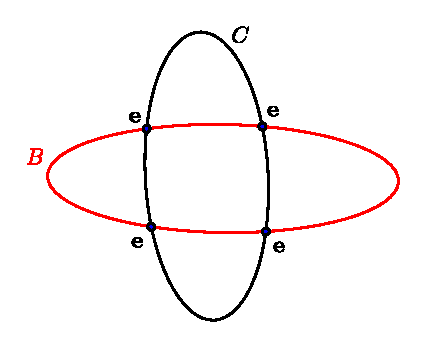
\includegraphics[scale=.6]{intersecao-C-B}
\caption{\textit{Epipolos que satisfazem as restrições de projeção e de calibração podem ser encontrados como as interseções das cônicas B e C.}}
\label{inter-B-C}
\end{figure}

Um epipolo ${\bf e}$ que gera uma cônica $B$ satisfaz à equação de décimo-sexto grau

\begin{equation}
{\bf e}^\top\,C\,{\bf e} = 0
\label{dezesseis}
\end{equation}
se, somente se, ele satisfaz às restrições de projetividade e de calibração. No caso em que a cônica $B$ pode se degenerar em um par de retas, a homografia $(\omega \cdot B)$ permuta as retas do par e assim, a equação \ref{dezesseis} descreve também seis retas passando por cada par dos quatro possíveis epipolos na imagem. Algebricamente, isso significa que a equação \ref{dezesseis} tem $|B|$ como um fator. Na figura \ref{plot-C} podemos observar duas plotagens da curva de dezesseis graus, uma com e outra sem a visualização dessas seis retas.

\begin{figure}[!htb]
\centering
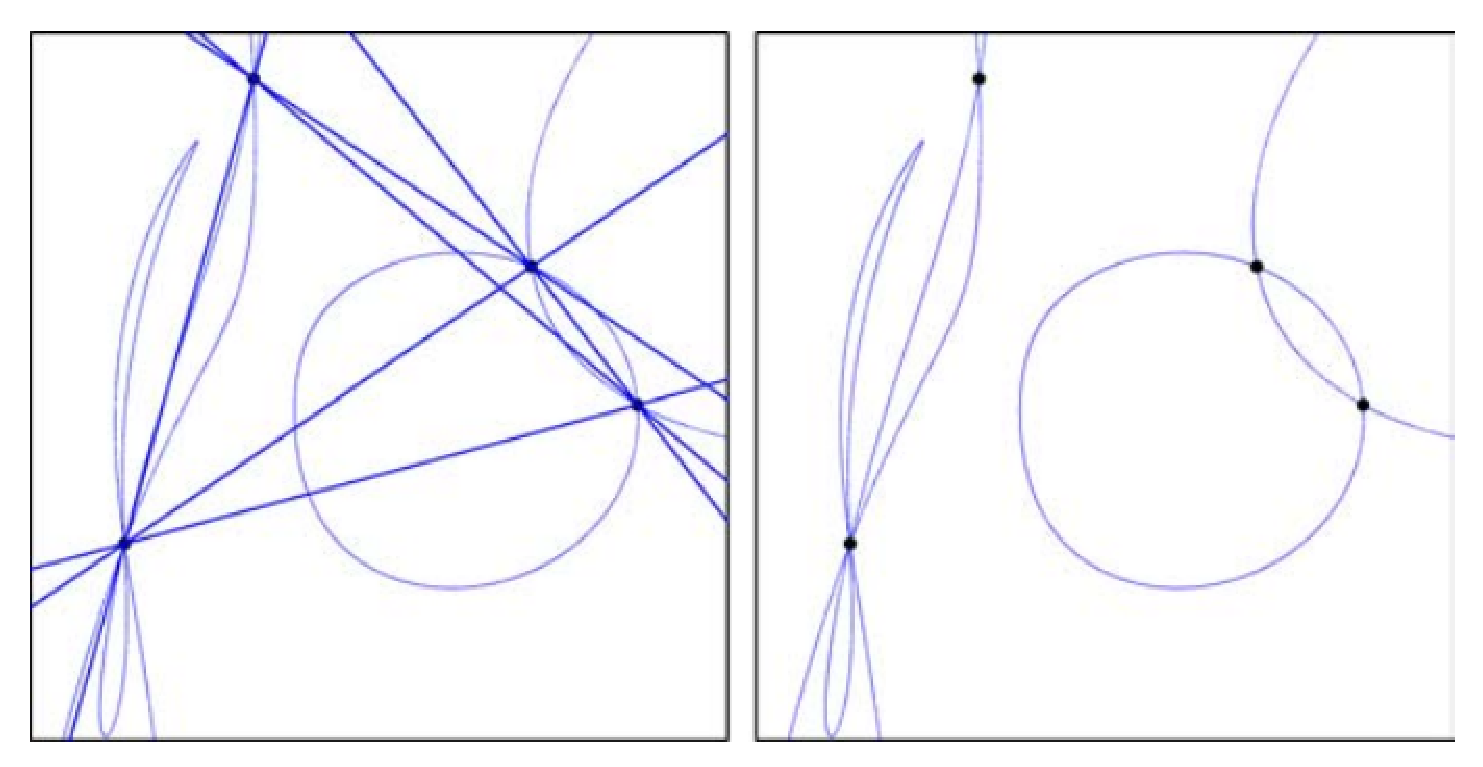
\includegraphics[scale=.6]{plotagem-C}
\caption{\textit{Podemos observar o lugar geométrico dos possíveis epipolos definido pela equação de décimo-sexto grau, a qual define (alem das curvas) as possíveis seis retas. A direita, a mesma imagem sem as retas.}}
\label{plot-C}
\end{figure}

Qualquer epipolo ${\bf e}$ para o qual $|B|\ne0$ satisfaz as restrições de projetividade e calibração se, e somente se, ${\bf e}$ satisfaz a equação de décimo grau remanescente de $e^\top\,C\,e=0$, ou seja, a equação restante após a eliminação do $|B|\ne0$. Geometricamente, temos que os pontos não podem se alojar em quaisquer das seis retas por conta da restrição de calibração. É possível remover $|B|\ne0$ da equação \ref{dezesseis} para se chegar à equação de décimo grau e o trabalho é algebricamente pesado mas também pode ser inteiramente encontrado em \cite{kneebone}. A curva de décimo grau é descrita pela equação

\begin{equation}
e^\top\,G\,e=0,
\label{dez}
\end{equation}
onde 
\begin{equation}
G=4\,U^\top\,D'^*\,B^*\,D'^*\,U-4\,t'^2\,B\,D\,D'^*\,(D\,B-t\,I)+s\,D^*-t^2\,t'^2\,D'^*
\label{conica-G}
\end{equation}
com as definições:

\begin{equation}
\begin{array}{rcl}
D&\equiv&\omega^*,\\
t&\equiv&tr(D\,B),\\
U&\equiv&(\omega \cdot B)\,\,\, \text{e}\\
s&=&(16\,|B|\,|D'|\,t'+t'4-4\,t'2\,tr(B*\,D'*)).
\end{array}
\end{equation}

A partir das consideraçoes feitas até aqui, podemos expor o principal resultado de \cite{kneebone}, o qual afirma que um ponto é um candidato a epipolo de acordo com as restrições de projetividade e calibração se, e somente se, satisfaz a equação de décimo grau definida em \ref{dez}. O que é equivalente ao fato de que ${\bf e}$ deve se alojar na cônica $G$ definida em \ref{camera-G}. Para um epipolo ${\bf e}$ qualquer na curva de décimo grau, o outro epipolo ${\bf e'}$ é calculado pela função de sétimo grau ${\bf e'} \sim U'*\,U\,{\bf e}$, dada em \ref{funcao-de-e}. Na figura \ref{curva-10} observamos alguns exemplos de curvas de décimo grau com seus possíveis epipolos. 

\begin{figure}[!htb]
\centering
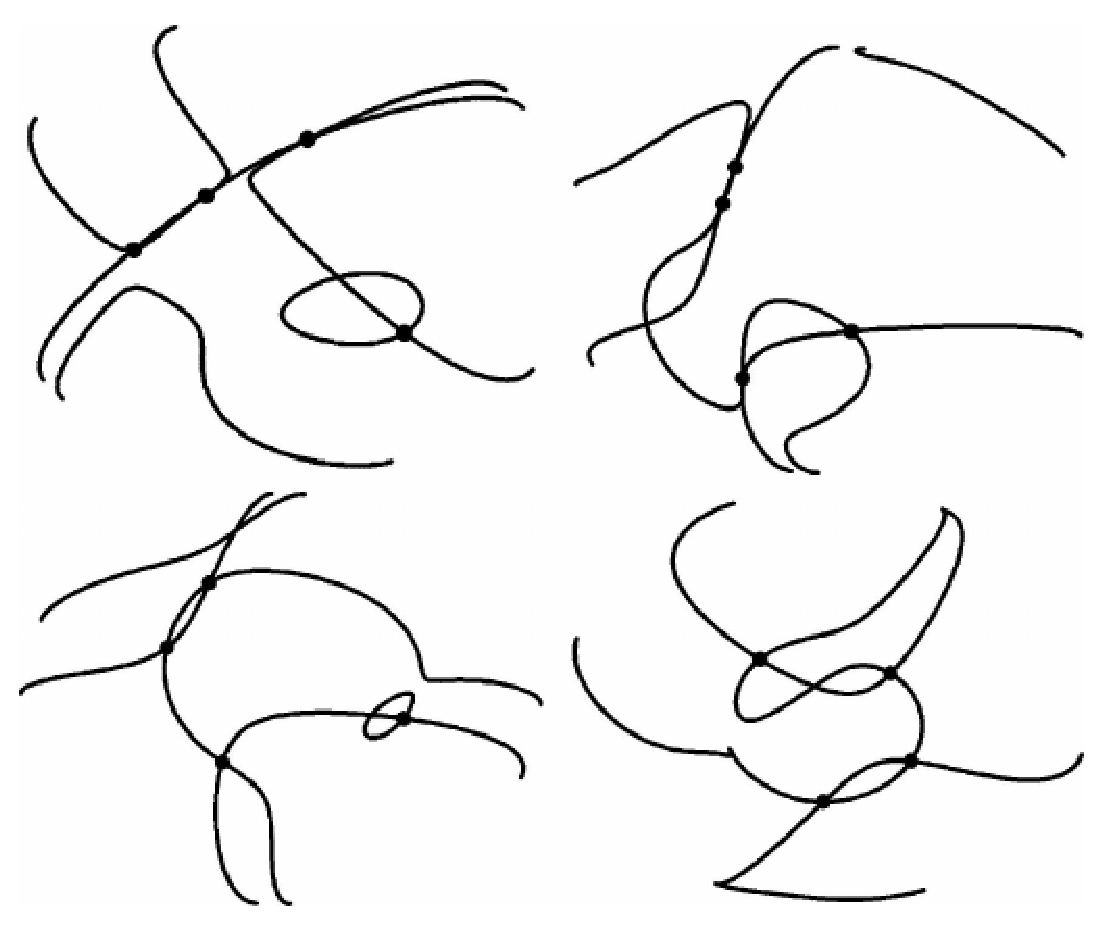
\includegraphics[scale=.85]{ex-curva-10}
\caption{\textit{Quatro exemplos de curvas de decimo grau definidas pela equaçao \ref{dez}, juntamente com seus respectivos epipolos.}}
\label{curva-10}
\end{figure}

Dado um ponto na curva de décimo grau, é importante verificar se o mesmo satisfaz a restrição de orientação, que é o fato de o correspondente ponto 3D no espaço situar-se em frente ao plano das duas imagens, conforme retratado na figura \ref{retr-orien}. Ou seja, o ponto no espaço 3D deve situar-se na metade da frente dos raios emanados de seus respectivos pontos nas duas imagens. Dado um epipolo ${\bf e}$ numa imagem, ${\bf e'}$ fica unicamente determinado pela equação \ref{funcao-de-e} na outra imagem. Após determinado o par de epipolos, a homografia da linha epipolar é unicamente definida pela correspondência desses pontos e assim determinamos a matriz essencial. Se ignorarmos uma diferença de escala considerando que a linha base que liga as duas câmeras tem comprimento unitário, temos que existem quatro configurações para a posição das duas imagens num sistema 3D. A restrição projetiva é satisfeita em quisquer dessas quatro configurações, pois os dois raios emanados do par de pontos correspondentes nas duas imagens continuam coplanares e devem se interseptar num ponto comum. A restrição de orientação é satisfeita exatamente quando os quatro pares de pontos correspondentes indicam a mesma configuração. Podemos dividir a restrição de orientação em duas partes: primeiro quando a homografia de reta epipolar é orientada, ou seja, quando os dois raios passando pelo par de pontos correspondentes nas imagens, estão no mesmo semiplano definido pela reta base onde se encontram as imagens (será chamada restrição de orientação epipolar); e segundo, a condição de que as duas metades dos raios que se projetam para a parte da frente devem convergir para um ponto comum (será chamada restrição de convergência).  

\begin{figure}[!htb]
\centering
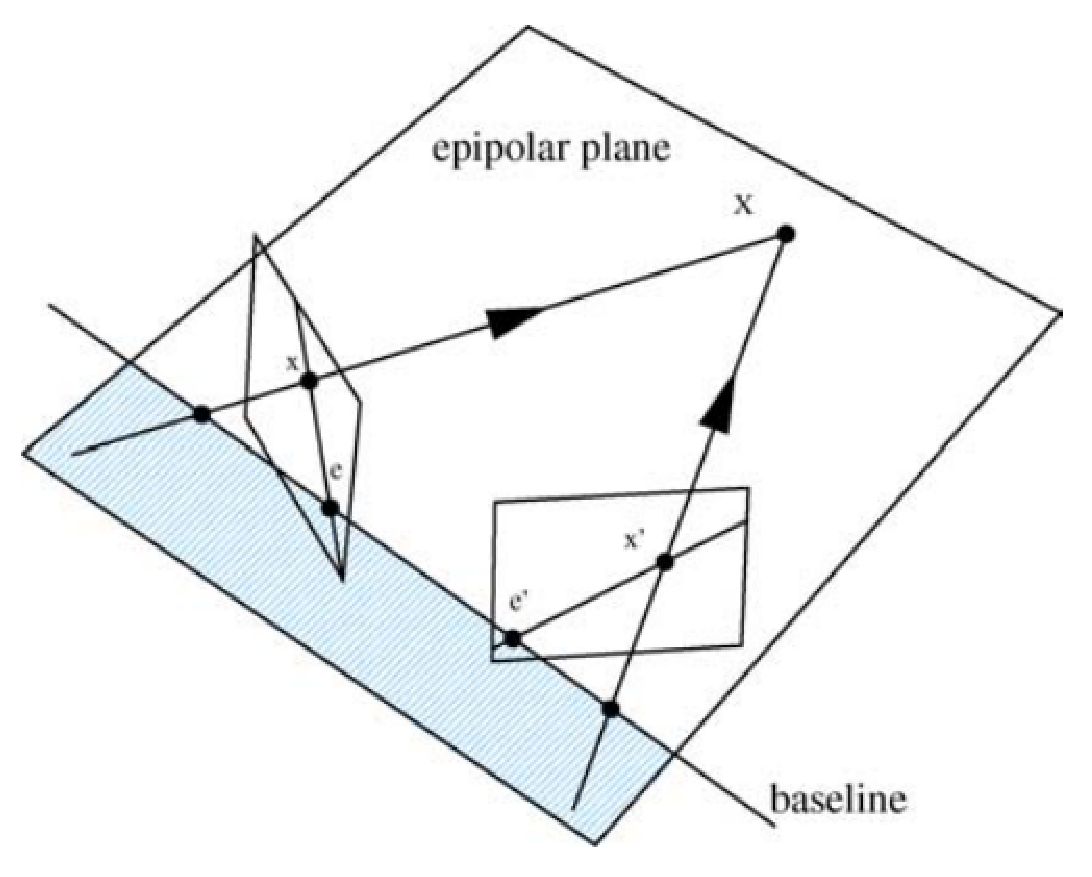
\includegraphics[scale=.85]{restricao-orientacao}
\caption{\textit{A restrição de orientação é simplesmente o fato de que o ponto no espaço 3D deve estar na parte da frente dos respectivos raios emanados de cada imagem.}}
\label{retr-orien}
\end{figure}

A restrição de convergência deve garantir que raios retroprojetados de cada imagem devem convergir. Isso não acontece somente se os raios forem paralelos e, uma forma de parametrizar, é através do ângulo formado entre o ponto na primeira imagem ${\bf x}$ e ${\bf e}$, e o ângulo entre o ponto na segunda imagem ${\bf x'}$ e ${\bf e'}$. Como a reta base passa por ${\bf e}$ e ${\bf e'}$, se os ângulos com os respectivos pontos forem iguais, os dois raios serão paralelos e não ocorrerá a convergência.


{\bf Aplicação da teoria no caso trifocal, com quatro pontos e três imagens.} As novidades do artigo se encontram, basicamente, no tipo de reconstrução 3D para duas imagens. A aplicação a seguir segue o padrão, até então convencional, de projetar as reconstruções na terceira imagem e minimizar o erro em relação aos dados já disponíveis. Assim, dados quatro pontos numa imagem e suas respectivas correspondências em outras duas imagens (todas com as câmeras calibradas), podemos escolher duas dessas imagens para traçarmos a curva de décimo grau de acordo com a esolha de um parâmetro $\theta$ que irá definir a cônica $B$, do feixe de cônicas, a ser utilizada.  Dada $B$ podemos calcular a cônica $G$ a partir da equação \ref{conica-G} como uma função de $B$, e as interseções de $B$ e $G$ podem ser determinadas como a solução de uma equação de quarto grau confrome descrito no apêndice do artigo. Assim, temos quatro soluções para   ${\bf e}$ e cada solução pode ser usada para calcular ${\bf e'}$ na segunda imagem de acordo com a equação \ref{funcao-de-e}. Note que para cada parâmetro $\theta$ teremos, a partir daqui, dezesseis caminhos a seguir. Com os epipolos encontramos a homografia da reta epipolar  e daí, a matriz essencial das duas imagens para cada uma das soluções. Existem vários métodos para reconstrução à partir da triangulação usando duas imagens, como por exemplo, \cite{nister5p2v} e \cite{Fabbri:Kimia:IJCV2015}. Conseguidas as reconstruções dos pontos 3D, existem também vários outros métodos de obtenção da câmera ralativa à terceira imagem, como por exemplo \cite{haralick} e \cite{bib:kuang}. Usados três pontos 3D para determinar a câmera da terceira imagem, podemos usar o quarto ponto para ser projetado na terceira imagem e comparar o resultado com o dado já obtido. Ou seja, para cada escolha do parâmetro $\theta$ (ou da cônica $B$), o procedimento consiste em minimizar um erro na imagem. Como o problema é supra restringido por um grau de liberdade, com os ruídos das correspondências, o valores encontrados para a reprojeção do quarto ponto não coincidirá com o dado observado mesmo que usada a correta solução. Como para cada $\theta$ escolhido teremos dezesseis configurações de câmera da terceria imagem e dezesseis reporjeções, todas essas reprojeções definem uma complexidade enorme de curvas na terceira imagem. Na figura \ref{curvas-f(theta)} é dada uma ideia da dificuldade extrema do problema envolvendo três imagens e quatro pontos. 

\begin{figure}[!htb]
\centering
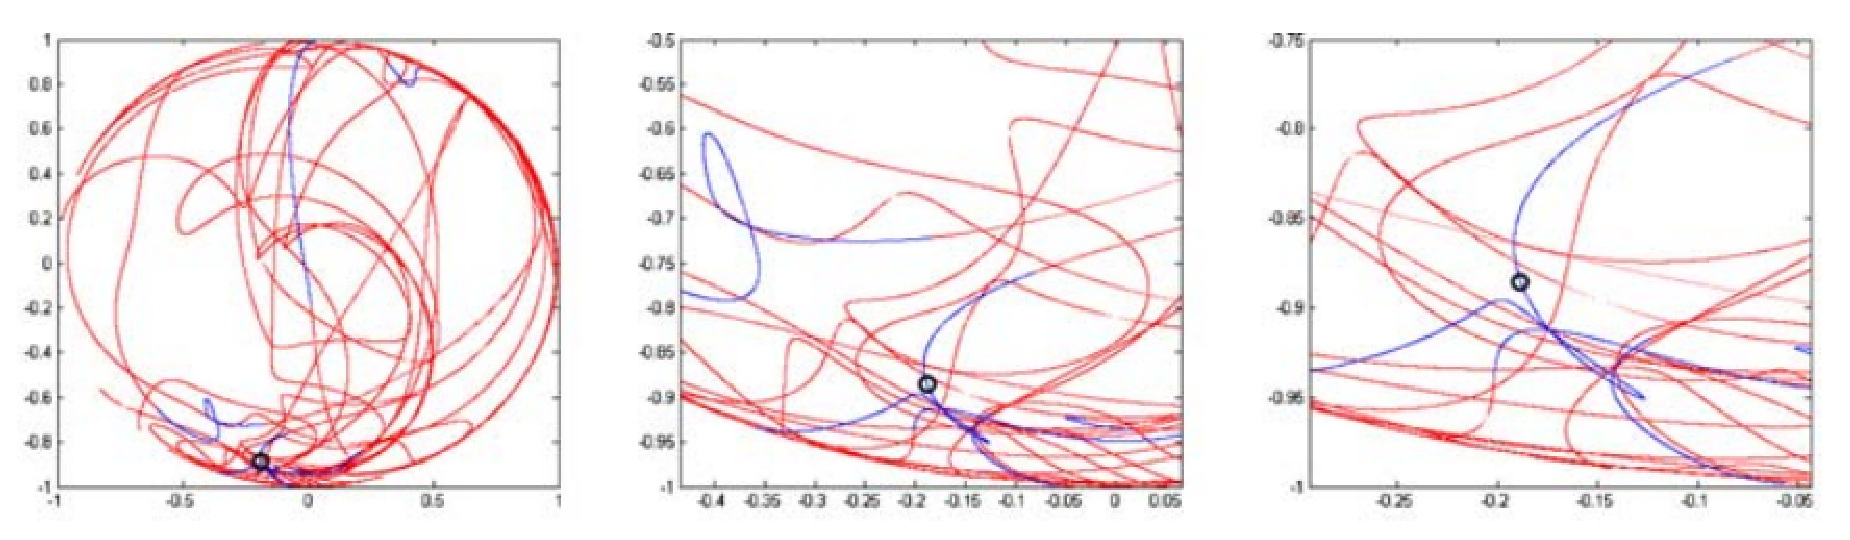
\includegraphics[scale=.52]{varias-curvas-f-theta}
\caption{\textit{A reprojeçao do feixe de conicas na terceira imagem e do quarto ponto reconstruido nos da uma ideia da dificuldade do problema de 3 imagens com quatro pontos.}}
\label{curvas-f(theta)}
\end{figure}

Para um grupo aleatório de quatro pontos, em geral a projeção da curva de décimo grau não passará pelos pontos. Antes de iniciar os cálculos, os pontos são co-registrados por uma homografia que será usada para transformar o DIAC  da segunda imagem no sistema de coordenadas da primeira. Existem várias maneiras de parametrizar o feixe de cônicas e uma delas é escolher duas cônicas dentre as degeneradas como base para o feixe.


